%
\documentclass[12pt,letterpaper]{article}

% The usual packages
\usepackage[left=1in,top=1in,right=1in,bottom=1in]{geometry}
\usepackage{setspace}
\usepackage{amsmath}
\usepackage{ntheorem}
\usepackage{longtable}
\usepackage{indentfirst}
\usepackage{qtree}
\usepackage{booktabs}
\usepackage{graphicx}
\usepackage{float}
\usepackage{fullpage}
\usepackage{endnotes}
\usepackage[sort]{natbib}
\citestyle{agsm}
\renewcommand\harvardand{and}
\usepackage{breakcites}
\usepackage{multirow}
\usepackage{tabulary}
\usepackage{rotating}

% Math
\newtheorem{hyp}{Hypothesis} 
\newcounter{subhyp} 
\newcommand{\subhyp}{ 
  \setcounter{subhyp}{0} 
  \renewcommand\thehyp{\protect\stepcounter{subhyp} 
  \arabic{hyp}\alph{subhyp}\protect\addtocounter{hyp}{-1}} 
} 
\newcommand{\normhyp}{ 
  \renewcommand\thehyp{\arabic{hyp}} 
  \stepcounter{hyp} 
} 
\newtheorem{lemma}{Lemma}
\newtheorem{proposition}{Proposition}
\newtheorem{theorem}{Theorem}
\newtheorem{claim}{Claim}
\newenvironment{proof}[1][Proof]{\begin{trivlist}
\item[\hskip \labelsep {\bfseries #1}]}{\end{trivlist}}
\newenvironment{definition}[1][Definition]{\begin{trivlist}
\item[\hskip \labelsep {\bfseries #1}]}{\end{trivlist}}
\newenvironment{example}[1][Example]{\begin{trivlist}
\item[\hskip \labelsep {\bfseries #1}]}{\end{trivlist}}
\newenvironment{remark}[1][Remark]{\begin{trivlist}
\item[\hskip \labelsep {\bfseries #1}]}{\end{trivlist}}

\long\def\symbolfootnote[#1]#2{\begingroup%
\def\thefootnote{\fnsymbol{footnote}}\footnote[#1]{#2}\endgroup}

%% Draft
% Title
\begin{document}
\begin{center}
{\LARGE Overcoming Structural Barriers: The Effect of Migrant Networks and Coordinated Financial Policies on International Investment}\\\vspace{2mm}
\vspace{3mm}
Kelly McCaskey\symbolfootnote[1]{Kelly McCaskey is a Ph.D. student in the Department of Political Science at Texas A\&M University (kellymccaskey@tamu.edu). 
%I'd like to thank Phil Arena, Austin Mitchell, Carlisle Rainey, Harvey Palmer, and my fellow panel participants at ISA 2015 for their helpful comments. I would like to especially thank Eric Hasbrouck for productive discussions in the early stages of this paper. Additionally, I would like to thank David Leblang for making his data publicly available. Replication materials can be found at: http://www.github.com/kellymccaskey/taxation.
\\\vspace{3mm}}
\end{center}

% Abstract
\begin{quote}
\begin{center} Abstract\end{center}
Migrant diaspora networks act as a conduit for international investment to their country of origin by lowering information asymmetries and transaction costs. I argue that these networks have a positive effect on both international portfolio investment, defined as cross-border investments both in equities and in short- and long-term bonds, and foreign direct investment and the strength of the effect is conditional upon the existence of a coordinated financial policy. In particular, I hypothesize that dual taxation treaties increase the positive effect of migrant diaspora networks on international portfolio investment but lead to little or no change in the positive effect of these networks on foreign direct investment. Using OECD and World Bank data for 2002, I find support for these hypotheses. These findings have policy implications for countries with high levels of emigration, by involving themselves in coordinated financial policies with countries containing large populations of their migrants, these countries should experience a greater inflow of international investment.
\end{quote}
% Remove page number from first page
\thispagestyle{empty}

% Start main text
\newpage
\doublespace
\section*{Introduction}
How do both formal and informal processes influence international investment? Formally, the growth in international institutions contributes to a decrease in both information and transaction costs. International institutions can produce coordinated financial policies that provide information about the type of state that is willing to sign such an agreement as well as the terms of the agreement. These can consist of types of trade agreements and the terms of such an agreement, if and how a currency may be pegged, whether it belongs to a particular currency union, or the investment tax policies in effect. 

Likewise, informal channels also influence information and transaction costs. Migrant diaspora networks serve as a path through which information is exchanged, thus creating opportunities for investment across pairs of countries \citep{Greif1989, Leblang2010, MadhavanIriyami2009, Vaaler2011}. A diaspora network is best defined as, ``a social collectivity that exists across state borders and that has succeeded over time to (i) sustain a collective national, cultural, or religious identity through a sense of internal cohesion and sustained ties with a real or imagined homeland and (ii) display an ability to address the collective interests of members of the social collectivity through a developed internal organizational framework and transnational links" (\citealt{AdamsonDemetriou2007}, 497). By positioning my argument as a combination of these formal and informal networks lowering these costs, I provide a more nuanced explanation. Positing that coordinated financial policies also play a role by further reducing information and transaction costs in combination with the diaspora network bridging the two countries, I explore other financial aftereffects of migration beyond remittances and foreign aid.  

%\citet{Leblang2010} finds that migrant diaspora networks act as a conduit for both portfolio and foreign direct investment across pairs of countries because these networks decrease informational costs to investors. 
In this case, I use the term coordinated financial policies to refer to trade agreements, tax treaties, and exchange rate policies, among others. Specifically, I contend that the effect of the migrant network is strengthened in combination with coordinated financial policies, creating greater opportunities for international investment. My analysis disaggregates international investment into international portfolio investment and foreign direct investment and uses the presence of a bilateral tax treaty, specifically a dual taxation treaty, as an indication of a coordinated financial policy. I argue that the strength of the effect of the diaspora network present in a country is conditioned by the presence of a dual taxation treaty and that this effect varies with regard to the type of investment. This varying strength is because of the nature of the types of investment, the type of information associated with and required for each, and the formal structural barriers that exist for each. 

%A dual taxation treaty is a bilateral tax treaty designed to prevent multinational corporations (MNCs) or private individuals from paying taxes on income earned from economic activity in a foreign country twice. Without such a treaty, income would be taxed once in the host country of the economic activity and again where the company or individual is permanently registered or a permanent resident \citep{Neumayer2007}. Bilateral tax treaties also serve as a means of relieving the inefficient allocation of investment across countries that can arise with international investment. Inefficient investment occurs when investment is diverted from areas where it is most useful and productive but taxed at a higher rate, to an area with a lower tax rate but fewer opportunities for growth. Governments generally use tax policies to affect the rate of return on capital, provide public goods, and capture some of the profits that would normally be repatriated to the MNC's home country. Investors would then base their decisions on the after-tax rate of return, not the gross rate of return. These treaties adjust the tax environment for investment by specifying the rate at which investments are taxed \citep{BlonigenDavies2002}.  

%Disaggregating international investment into either international portfolio investment or foreign direct investment (FDI) allows us to more accurately differentiate how diaspora networks actually work to decrease information asymmetries and transaction costs. I define international portfolio investment as cross-border investments both in equities and in short- and long-term bonds. FDI refers to acquisition or creation of some element along the production supply chain by an MNC and can be either horizontal or vertical. 

%Horizontal FDI refers to ``an arrangement where a firm maintains production facilities in multiple countries, and each facility transforms raw or intermediate inputs into more finished products, often for sale in the local (domestic) market," while vertical has ``at least two stages of production and can be geographically separated to take advantage of location-specific differences in factor endowments," (\citealt{ButheMilner2008}, 744). The International Monetary Fund (IMF) categorizes an investment as FDI when it is large enough to give the parent firm some control over the management of the operation, specified as ownership of at least 10\% of the firm \citep{Jensen2003}. 

% As the associated information and transaction costs are substantially higher, \citet{Leblang2010} hypothesizes that migrant networks are more important for FDI than international portfolio investment. With his evidence to support this claim, I think the argument is more nuanced than that. I posit that the strength of the effect of the diaspora network present in a country is conditioned by the presence of a dual taxation treaty and that this effect varies with regard to the type of investment. This is because of the nature of the types of investment, the type of information associated with and required for each, and the structural barriers that exist for each. 

I proceed in four steps. First, I introduce how migrant networks serve as informal channels through which both information and transaction costs decrease for both international portfolio investment and FDI. Second, I discuss how the strength of the effect of the migrant network depends on the existence of a coordinated financial policy, likewise how a coordinated financial policy lowers information costs in a formal manner. Third, I develop and empirically test two interaction models. I find migrant networks do have a positive effect on both international portfolio investment and FDI but that dual taxation treaties increase this positive effect only on international portfolio investment. I conclude with a discussion of these results and of the broader implications of this analysis. 

\section*{Theory}
\subsection*{Migrant Networks as Information Channels}
Previous research identifies two aggregate level ways that migrant networks influence investment: through increased familiarity and through a decrease in informational asymmetries \citep{Leblang2010, Vaaler2011}. These two channels can be used by migrant networks separately and in combination to facilitate cross-border investment. The nature of portfolio investment and FDI are inherently different, so while each might respond to increased familiarity in a similar way, they may take advantage of informational asymmetries in different ways.

This familiarity effect refers to the emergence of beliefs about the economic values of an ethnic group analogous to product branding where members of the migrant network provide signals to investors that enable them to make inferences about the productivity of the business culture \citep{KapurMcHale2006, Vaaler2011, MadhavanIriyami2009}. Examples of increased familiarity can be seen in both a propensity to not internationally diversify stock portfolios and a preference for home-country products \citep{Gould1994, GrinblattKeloharju2001}. Generally known this is thought of as a ``home-bias," or a systematic preference for assets that are available in local markets as compared to those abroad \citep{CovalMoskowitz1999, CovalMoskowitz2001, Lewis1999}. 

Explanations for home bias rely on patterns of investor behavior. Investors may not evaluate the relative risks of different investments solely on their historical returns and have a tendency to attribute extra risk to foreign investments because they have less knowledge about these foreign markets, institutions, and firms. \citet{FrenchPoterba1991} find that the gains from diversification depend on the correlation of returns across different equity markets and the fact that investors have a tendency to expect domestic returns to be systematically higher than those associated with a more diversified portfolio. \citet{ShillerKonyaTsutsui1991} surveyed American and Japanese portfolio managers and found that while the Japanese were slightly more optimistic about both markets, the Americans and Japanese were each relatively more optimistic about their own market. 

We see similar outcomes in experiments investigating judgements about probability and risk-taking in non-investment settings as well. \citet{HeathTversky1991} present evidence of households behaving as if unfamiliar gambles are riskier than familiar ones, even when the two options have identical probability distributions. The primary explanation for an equity home bias is that domestic equities provide a better hedge for risks and we already know that investors are more likely to hedge their bets on something that is more familiar to them \citep{Lewis1999}. Migrant networks provide that increased familiarity for investors to make confident, informed decisions.

A decrease in information asymmetries helps investors to decrease the transaction costs associated with investment in foreign securities and the costs of doing business abroad. Transaction costs are said to hinder international diversification and bias stock portfolios toward those that are domestic or, at the very least, familiar to the investor \citep{TesarWerner1995}. I use transaction costs to cover both cultural and structural barriers including language, common business practices, institutional and regulatory differences, and the cost of obtaining information about institutional and regulatory differences. Migrant networks can provide knowledge of on-the-ground conditions and opportunities that would be costly and time-consuming for investors to discover independently \citep{Rauch2001}.

\begin{hyp}
An increase in migrant stock leads to an increase in international portfolio investment, whether or not there is a dual taxation treaty. 
\end{hyp}
 
Much like portfolio investment, we would expect migrant networks to promote FDI as well. \citet{Leblang2010} attributes this to the many different ownership stakes across a ``countless number of commodity classes," for foreign direct investors (p. 855). Knowledge provided by migrants helps to match investors in the host country with appropriate foreign opportunities. This kind of heads-up into the market is invaluable for FDI as it is generally associated with a long-term vision and higher relocation costs than necessary for portfolio investment \citep{ButheMilner2008}. Investors looking to use their capital abroad, particularly in a more concrete fashion than stocks and bonds, need a substantial amount of information prior to investing. So, consistent with \citet{Leblang2010}, I hypothesize that because they create increased familiarity and decrease informational asymmetries between potential markets, migrant networks are a vital asset to the decision-making process. 

\begin{hyp}
An increase in migrant stock leads to an increase in FDI, whether or not there is a dual taxation treaty. 
\end{hyp}

As MNCs are the primary source of FDI, in contrast to portfolio investment by private individuals, I expect this positive relationship between FDI and migrant networks to be weaker than that of portfolio investment. This weak relationship, relative to migrant networks and portfolio investment, is because of the differing economies of scale. Firms would already have lower transaction costs than individuals because there are more resources available to them \citep{Jensen2003}. For example, a firm looking to expand into China would not rely on migrant networks for language help, they would be able to hire someone who is already fluent in Mandarin, whereas a private individual looking to internationally diversify their portfolio would benefit from the knowledge of a migrant network in a similar situation. 
 
\subsection*{The Presence of Coordinated Financial Policies}

Another potential explanation for a home-bias in both portfolio investment and FDI is that taxes tend to disfavor foreign investors \citep{TesarWerner1995}. Investors can be subject to foreign withholding taxes on dividends from foreign investment, making their investment more inefficient. An efficient allocation of capital, for example, requires ``that capital be allocated between the two countries such that the rates of return are equal (or that all the capital invested in the high-return country)," (\citealt{BlonigenDavies2002}, 3). In order to make international investment more efficient, bilateral investment treaties are introduced. These treaties generally serve as a way to promise foreign investors nondiscriminatory rights and grant them specific individual rights in the country of investment \citep{ButheMilner2009}. There are two reasons for narrowing the focus on bilateral investment treaties to dual taxation treaties: (1) we can examine barriers to investment on a very basic level and (2) dual taxation treaties are bilateral, rather than multilateral, which makes their conditional effect on migrant networks directly observable. I have already hypothesized that migrant networks serve as a means for increasing investment through increased familiarity and decreased information costs so it would follow that a decrease in structural barriers would heighten the influence of the migrant networks. We can think of a dual taxation treaty as a key to a door; migrant networks provide the knowledge that there is a party going on behind the door, making it attractive to want to get inside, but you can`t if the door is locked. You can join the party only when the door is unlocked, and assuming you want to be with those inside.

The main purpose of a dual taxation treaty is to create a favorable investment atmosphere by excluding the possibility that the investor will be taxed on revenue in both their home country and the country of their investment. \citet{BlonigenDavies2004} list four primary functions of dual taxation treaties: standardizing tax definitions of treaty partners, reducing forms of tax avoidance, preventing treaty shopping, and providing relief from double taxation and rules reducing the maximum allowable withholding taxes on remitted income. Remitted income refers to dividend payments, interest payments, and royalty payments; the first two play an obvious role in international portfolio investment. Knowing that dual taxation treaties promote investment by reducing the uncertainty about the tax environment and by lowering structural barriers. So, there is good reason to posit that the combination of migrant networks and dual taxation treaties have a greater influence on international portfolio investment together than separately.

\begin{hyp}
A dual taxation treaty increases the positive effect of migrant stock on international portfolio investment. 
\end{hyp}

Previous studies on the determinants of FDI imply that FDI and portfolio investment should not be expected to behave similarly with regard to high-level economic policies \citep{Ahlquist2006}. Following prior understanding about international portfolio investment, we might think that a dual taxation treaty would have a positive effect on international investment of any type but previous research has demonstrated that this is not the case. \citet{Dagan2000} argues that the promotion of investment efficiency plays a very small role in treaty formation. He points out that treaties are more likely intended to reduce administrative costs, reduce tax evasion, and to extract tax concessions from treaty partners. \citet{Radaelli1997} agrees, positing that treaties are not so much geared toward promoting efficient investment but maximizing investor profits. 

Additionally, some of the tax benefits provided by the dual taxation treaty are irrelevant for expanding MNCs in the first place. First, MNCs would already be avoiding double taxation through contracts and other legal documents, and second, it is often much cheaper to expand an overseas venture with retained earnings than through repatriated and re-exported funds \citep{Hartman1985, Sinn1993}. \citet{BlonigenDavies2002} find some of the first empirical support that dual taxation treaties don't have much of an effect on FDI. Using OECD data spanning from 1983 to 1992, they find evidence demonstrating that dual taxation treaties have a negligible effect on FDI. Given this previous research, I don't expect that the effect of migrant stock on FDI will vary much between countries with a dual taxation treaty and those without. Migrant networks should be important to international investment regardless of the presence of a dual taxation treaty. %However, if the sample size is limited to exclude either all dyads where the investment source countries contain the headquarters of one of the top 100 MNCs or all dyads where the investment destination country is considered a resource curse country or one where GDP is tied to the extraction of natural resources, we would expect the effect to be greater than the sample as a whole of FDI dyads but smaller than that for portfolio investment, yet still not statistically significant.\citep{Ross1999}.\footnote{The samples are kept separately for the empirical analysis for the exclusion of both categories leaves a sample size too small for reliable estimates. See Tables \ref{tab:fdi-nomnc} and \ref{tab:fdi-norc} in Appendix B.}

\begin{hyp}
The effect of migrant stock on FDI should be similar in countries with and without a dual taxation treaty. 
\end{hyp}
 
I consider an increase or decrease of 0.10 of a percentage point of FDI in the presence of a dual tax treaty to be the minimum substantively meaningful effect. To determine the minimum substantively meaningful effect, I'll use an example of Lithuanian migrants in Belgium, a dyad that has a dual taxation treaty while containing the median amount of migrant population. In 2002, FDI from Belgium to Lithuania was approximately 1.4 million US-dollars (OECD). An increase or decrease of 0.10 of a percentage point would be the equivalent of an increase or decrease of \$1407, an essentially negligible amount. 
 
%According to the 2000 United States Census, there were approximately 1.3 million people in the United States identifying as Filipino \nocite{USCENSUS} and in 2002, United States FDI outflows to the Philippines were roughly 391 million dollars \citep{ASEAN}. In this situation, an increase or decrease of 0.10 percentage points in FDI would be the equivalent of about \$39,168; a negligible amount of money in the global economy.
 
My argument takes the form of the standard international capital asset pricing model (ICAPM) which predicts that investors should hold domestic assets in their portfolio that are proportional to their country's share of global capital market capitalization in the absence of information asymmetries and transaction costs \citep{LaneMilesi-Ferretti2004, Lewis1999, PortesRey2005}. Gravity models of international trade hold that bilateral transactions are a positive function of the size of the two economies and a negative function of the distance between them \citep{Lane2005, LaneMilesi-Ferretti2004, Leblang2010, LounganiModyRazin2002}. Previous studies have proxied for geographical distance and similarities, both cultural and otherwise, by the inclusion of variables such as a common language, a common border, a common colonial heritage, and bilateral telephone volume \citep{EichengreenLeungnaruemitchai2006, LaneMilesi-Ferretti2004, PortesRey2005, RoseSpiegel2008} which I also do. I demonstrate a deeper understanding of the positive relationship between migrant networks and international investment by arguing that the effect of migrant networks is conditional upon the presence of a dual taxation treaty and varies with regard to the type of investment.
 
\section*{Data and Measures}
Using data from \citet{Leblang2010}, I estimate two interaction models, one for each category of international investment, to test my hypotheses.\footnote{
%\baselineskip=2\normalbaselineskip 
See Appendix A for a detailed description of the data and variables.} Equation 1 estimates the modifying effect of dual taxation treaties for the first dependent variable, \emph{IPF}. \emph{IPF} measures international portfolio investment by the amount, in millions of US dollars, of bilateral cross-border investments in equities and short- and long-term bonds, for 56 source countries and 154 destination countries. The transactions, from data collected by the IMF, have been broken down by the country issuing the stock or bond. \emph{Migrant Stock} measures the total number of migrants from the destination country of investment residing in the source country of investment. This measure comes from a World Bank project on South-South migration and remittances. \emph{DTT} is a dichotomous variable with a value of 1 indicating that a dual taxation treaty exists within the dyad and a 0 otherwise. \emph{Migrant Stock $\times$ DTT} is the interaction term allowing the effect of migrant stock to vary with the presence or absence of a dual taxation treaty. \emph{Controls} represents the control variables and $\epsilon$ our error term.%\footnote{
%\baselineskip=2\normalbaselineskip 
%Control variables include: \emph{ln(GDP*GDP)} measured in dollars, representing the dyad's market size; \emph{ln(distance)} measured in kilometers; \emph{Growth Correlation} calculated as the correlation of the GDPs in the dyad on based on a five year moving average, which is then lagged five years; \emph{ln(Bilateral Telephone Volume)} as a measure of the volume of telephone traffic between the two countries to represent the exchange of information; \emph{Preferential Trade Agreements} and \emph{Contiguous Borders} as a dichotomous variables, 1 if present and 0 otherwise and an additive composite measure of similarity among the dyad which includes \emph{Common Language}, \emph{Common Currency},  \emph{Common Legal Heritage}, and \emph{Common Religion} with each weighted equally}

The control variables include: \emph{ln(GDP*GDP)} measured in dollars, representing the dyad's market size; \emph{ln(Distance)} measured in kilometers; \emph{Growth Correlation} calculated as the correlation of the GDPs in the dyad on based on a five year moving average, which is then lagged five years; \emph{ln(Bilateral Telephone Volume)} as a measure of the volume of telephone traffic between the two countries to represent the exchange of information; \emph{Preferential Trade Agreements} and \emph{Contiguous Borders} as a dichotomous variables, 1 if present and 0 otherwise and an additive composite measure of similarity among the dyad. This similarity measure includes \emph{Common Language}, \emph{Common Currency},  \emph{Common Legal Heritage}, and \emph{Common Religion}, measured dichotomously with each equally weighted. I include this composite measure to obtain more precise estimates by reducing the introduction of multicollinearity into my model. The results of the fully specified model can be found in Appendix B. 

\begin{align}
\nonumber IPF = \beta_{cons} &+ \beta_{Migrant}Migrant Stock + \beta_{DTT}DTT \\
\nonumber &+ \beta_{Migrant \times DTT}Migrant Stock \times DTT\\
 &+ \beta_{Controls}Controls +\epsilon 
\end{align}
\indent I use Equation 2 to estimate the modifying effect of dual taxation treaties for the second dependent variable, \emph{FDI}. \emph{FDI} measures bilateral FDI, in millions of US dollars, from 28 Organization for Economic Cooperation and Development (OECD) source countries and 158 (both OECD and non-OECD) destination countries. The remaining terms are the same as in Equation 1. 
\begin{align}
\nonumber FDI = \beta_{cons} &+ \beta_{Migrant}Migrant Stock + \beta_{DTT}DTT \\
\nonumber &+ \beta_{Migrant \times DTT}Migrant Stock \times DTT\\
 &+ \beta_{Controls}Controls +\epsilon 
\end{align}\label{eqn:2} 
The effect of migrant stock on portfolio investment is given by:\nocite{BramborClarkGolder2006} 
\begin{eqnarray}
\frac{\partial IPF}{\partial Migrant Stock} =  \beta_{Migrant} + \beta_{Migrant \times DTT}DTT
\end{eqnarray}

\noindent where the effect is conditional on the presence of a dual taxation treaty.\footnote{
%\baselineskip=2\normalbaselineskip 
The equations for the standard errors of the marginal effects can be found in Appendix B.}  The effect of migrant stock in the absence of a dual taxation treaty is given by the coefficient for migrant stock while the sum of the coefficient for migrant stock and the product term in the presence of a dual taxation treaty determines the effect with a dual taxation treaty. 

A similar equation is used to estimate the effect of migrant stock on FDI:
\begin{eqnarray}
\frac{\partial FDI}{\partial Migrant Stock} =  \beta_{Migrant} + \beta_{Migrant \times DTT}DTT
\end{eqnarray}

%Following \citet{Leblang2010}, 
I use fixed-effects ordinary least squares (OLS) and two-way clustering of standard errors, clustered on the investment source and destination country \citep{BerryGolderMilton2012, Zeileis2006, CameronGelbachMiller2006}. I am restricted to using cross-sectional data rather than time-series because the migrant data only exists for 2002. %\footnote{I did not simultaneously estimate a seemingly unrelated regression because of the difference in sample sizes of portfolio investment and FDI. See Appendix B for results.}
%\footnote{
%\baselineskip=2\normalbaselineskip 
%I have omitted the \emph{Genetic Distance} variable from \citet{Leblang2010}'s original dataset. \emph{Genetic Distance} was developed as a measure of genetic distances between indigenous populations through differing DNA characteristics in the human population and was provided by Spoloare and Wacziarg in their 2008 paper. \citet{Leblang2010} ran several models and listwise deleted those observations in which \emph{Genetic Distance} was missing. I was unable to merge their variable with the rest of \citet{Leblang2010}'s dataset, and so proceeded without it \citep{Kingetal2001}. My estimates were similar after adding the new observations that were previously missing due to the \emph{Genetic Distance} variable.} 
Tables 1 and 2 provide the estimates and 90\% confidence intervals for the two models.%\footnote{See Appendix B for results with the non-composite measure of similarity.}%\footnote{\baselineskip=2\normalbaselineskip My estimates are robust to alternative estimation techniques, see Appendix B for more information.}

\section*{Results}
\subsection*{Migrant Networks and Portfolio Investment}
In estimating the models, I find support for all four of my hypotheses. Migrant diaspora networks promote international investment by increasing familiarity and reducing information costs. The results in Table \ref{tab:ipf} provide evidence for my first hypothesis, that an increase in migrant stock leads to an increase in international portfolio investment regardless of the existence of a dual taxation treaty. Migrant networks serve as a means for exchanging particular pieces of information that would be helpful to investors, such as common business practices and institutional and regulatory differences.

To provide some substantive context to my findings, we can focus, again, on the example of Lithuania and Belgium. This dyad contains both the median number of migrants (Lithuanian migrants into Belgium) and a dual taxation treaty. Following this first hypothesis, the coefficient indicates that if Belgium experienced a 1 percentage point increase in the Lithuanian migrant population, roughly 1100 people, Lithuania would experience a 0.18 percent increase in international portfolio investment from investors in Belgium, regardless of whether or not a dual taxation treaty exists between Belgium and Lithuania. In 2002, this would have been an increase of about \$3.5 million.

Not only does a migrant network promote international portfolio investment on its own, but the strength of its effect increases substantially in combination with a dual taxation treaty. Dual taxation treaties can lower information asymmetries in the case of international portfolio investment though the harmonization of tax policies and the lowering of structural barriers through its very existence. I find empirical support that the significant, positive effect of migrant networks on international portfolio investment is even stronger in countries where a dual taxation treaty exists. In fact, the presence of a dual taxation treaty should increase the effect of migrant stock on international investment almost threefold. In the Belgium-Lithuania example, we would expect to experience about a total of 0.39 percentage points more investment, an increase of about \$15 million, with the combination of a migrant network and a dual taxation treaty than if there were no dual taxation treaty. This is illustrated in Figure 1.  
\begin{singlespace}
\begin{table}[h]
\begin{center}
\caption{Migrant Stock and International Portfolio Investment} \label{tab:ipf}
\begin{tabular}{lcccc}
\toprule	
Variable    & Coef. & 90\% C.I.  & Coef. & 90\% C.I \\
\hline
Constant      &-135.15	&[-206.03, -64.27] & -121.44 &[-189.99 , -52.89]\\
Migrant Stock	&0.18	&[0.09, 0.27] &0.12	&[0.02, 0.21]\\
Migrant Stock $\times$ Dual Taxation &- 	&- &0.27	&[0.15, 0.38]\\
Market Size     	&0.17	&[0.08, 0.25] &0.16   	&[0.08, 0.24]\\
Distance     	&-1.15	&[-1.49, -0.81]  &-1.16  	&[-1.49, -0.83]\\
Contiguous Border 	&-0.88	&[-1.48, -0.28]	&-1.08  	 &[-1.64, -0.52]\\
Growth Correlation 	&0.06	&[-0.19, 0.31] &0.04	&[-0.20, 0.28]\\
Dual Taxation Treaty	&1.29	&[0.80, 1.78] &-0.40	&[-1.22, 0.42] \\
PTA	 	&0.87	&[0.21, 1.52] &0.79	&[0.19, 1.40]	\\ 
Bilateral Telephone Volume	&0.09	&[0.00, 0.17] &0.08	&[0.00, 0.16]\\
Dyad Similarities	&0.32	&[0.19, 0.45]	&0.31	&[0.18, 0.44]\\

\\N &5134 	&	&5134	&\\
$R^{2}$ &0.79	&	&0.79	& \\
\hline
DV: log(portfolio investment)\\
\bottomrule
\end{tabular}
\end{center}
\end{table}
\end{singlespace}

%\newpage
\begin{figure}[h]
\begin{center}
\includegraphics[scale = 0.60]{figs/me-comparison.pdf}
\singlespace{\caption{\small{The marginal effect is represented by a solid dot. The purple solid lines indicate the 90\% confidence interval around the marginal effect of a dyad without a dual taxation treaty while the orange dotted lines indicate that for a dyad with a dual taxation treaty. The plot on the left demonstrates the marginal effect of migrant stock on international portfolio investment in countries with and without a dual taxation treaty. This shows that the marginal effect of migrant stock is about three times greater where a dual taxation treaty is present. The plot on the right shows that there is no meaningful difference in the marginal effect of migrant stock on FDI with or without a dual taxation treaty.}}}
\label{fig:me}
\end{center}
\end{figure}

%\newpage
\subsection*{Migrant Networks and FDI}
We see a similar effect on FDI outflows. I expect that migrant networks greatly increase business opportunities for investors in their new country of residence in their homeland by possessing the ability to provide important on-the-ground information. This makes it easy for investors to acquire information and leads me to expect support for the second hypothesis: an increase in migrant stock leads to an increase in FDI, whether or not there is a dual taxation treaty. The model in Table \ref{tab:fdi} estimates indicate that migrant networks do, in fact, have a positive effect on FDI. In continuing our Belgium-Lithuania example, a one percent increase in migrant stock would lead to a 0.19 percentage point increase in Belgian FDI to Lithuania, or about \$3.7 million, regardless of whether or not a dual taxation treaty is in place. This is, as we predicted, slightly less than the effect that migrant networks had on portfolio investment. This is most likely due to the additional resources that can be used toward information gathering that MNCs have in comparison to private individuals and their portfolio investments.

%\newpage
\begin{singlespace}
\begin{table}[h]
\begin{center}
\caption{Migrant Stock and FDI} \label{tab:fdi}
\begin{tabular}{lcccc}
\toprule	
Variable    & Coef. & 90\% C.I.  & Coef. & 90\% C.I \\
\hline
Constant      &-116.82	&[-191.85, -41.78]	&-117.34	&[-193.6, -50.2]\\
Migrant Stock	&0.19	&[0.09. 0.29]	&0.19	&[0.09, 0.29]\\
Migrant Stock $\times$ Dual Taxation &-	&-	&-0.007	&[-0.09, 0.08]\\
Market Size      &0.15   	&[0.06, 0.23]     &0.15	&[0.07, 0.23] \\
Distance      &-1.21  	&[-1.59, -0.84]      &-1.22	&[-1.58, -0.84]\\
Contiguous Border &0.68  	 &[-0.09, 1.44] 	&0.68	&[-0.09, 1.44]      \\
Growth Correlation &0.19	&[0.17, 0.21] 	&0.20	&[-0.05, 0.43]\\
Dual Taxation Treaty	&0.66	&[0.18, 1.13] 	&0.71	&[0.00, 1.41]\\
PTA	&0.09	&[-0.53, 0.72] 	&0.09	&[-0.53, 0.72]\\ 
Bilateral Telephone Volume	&-0.04	&[-0.16, 0.07] 	&-0.04	&[-0.16, 0.07]\\
Dyad Similarities	&0.51	&[0.32, 0.71]	&0.51	&[0.32, 0.70]\\

\\N &3658 	&	&3658	&\\
$R^{2}$ &0.64	&	&0.64	& \\
\hline
DV: log(FDI) \\
\bottomrule
\end{tabular}
\end{center}
\end{table}
\end{singlespace}

%\newpage
As consistent with expectations, the difference in the marginal effects of migrant stock across countries with and without a dual taxation treaty on FDI appears to be both statistically insignificant and negligible, as demonstrated in the right panel of Figure 1.  As FDI is more heterogenous than international portfolio investment, it requires different types of information. Dual taxation treaties do not provide the kind of tax benefits that promote efficient FDI the same way that they do for international portfolio investment. Additionally, much of the earnings from FDI are not repatriated, but rather reinvested into the continuation of the overseas venture. I find the effect of migrant stock on FDI is substantively similar across systems with and without a dual taxation treaty. \citet{Rainey2014} shows that using two one-sided tests against some substantively meaningful value allows researchers to make a more compelling argument of negligible effects. Following his example, I have set our minimum substantively meaningful effect to an increase or decrease of 0.10 percentage points. The 90\% confidence interval of our estimate ranges from -0.09 to 0.08 percentage points, falling into the range of negligible effects and supporting my hypothesis. 

\begin{singlespace}
\begin{table}[h]
\begin{center}
\caption{Migrant Stock and FDI - Excluding All Source Countries Containing a Top 100 MNC Headquarter} \label{tab:fdi-nomnc}
\begin{tabular}{lcccc}
\toprule	
Variable    & Coef. & 90\% C.I.  & Coef. & 90\% C.I \\
\hline
Constant      &-146.04	&[-193.42, -98.67]	&-145.39	&[-193.19, -97.59]\\
Migrant Stock	&0.37	&[0.29, 0.45]	&0.36	&[0.27, 0.44]\\
Migrant Stock $\times$ Dual Taxation &-	&-	&0.01	&[-0.07, 0.09]\\
Market Size      &0.18	&[0.13, 0.23]      &0.18	&[0.13, 0.23] \\
Distance      &-1.17  	&[-1.50, -0.84]     &-1.17  	&[-1.50, -0.84]\\
Contiguous Border &0.30  	 &[-0.51, 1.11] 	&0.29  	 &[-0.51, 1.10]     \\
Growth Correlation &0.23	&[-0.08, 0.54] 	 &0.23	&[-0.08, 0.54] \\
Dual Taxation Treaty	&0.76	&[0.33, 1.18] 	&0.71	&[0.02, 1.40] \\
PTA	&0.47	&[-0.11, 1.05] 	&0.46	&[-0.13, 1.05] \\ 
Bilateral Telephone Volume	&-0.07	&[-0.23, 0.09] 	&-0.07	&[-0.23, 0.09] \\
Dyad Similarities	&0.55	&[0.37, 0.73]	&0.55	&[0.37, 0.71]\\

\\N &2320 	&	&2320	&\\
$R^{2}$ &0.62	&	&0.62	& \\
\hline
DV: log(FDI) \\
\bottomrule
\end{tabular}
\end{center}
\end{table}
\end{singlespace}

Because it would be impossible to disaggregate the investment coming from large MNCs, excluding the source countries which contain the headquarters of one of the 100 largest MNCs is one way to examine the conditioning effect of dual taxation treaties on the strength of a migrant network\footnote{The list of sample countries can be found in Appendix A.}. I would expect the conditioning effect of a dual taxation treaty to be greater than that for the full FDI sample, but still less than that for portfolio investment, for the exclusion sample. While large MNCs would typically have the information costs alleviated by a dual taxation treaty built into their business model, smaller companies doing business abroad may not and this is where we would see the conditioning effect. Table \ref{tab:fdi-nomnc} displays these results. This estimate still falls within our range of negligible effects, however, it is now positive and larger than that of the full FDI sample.

\begin{singlespace}
\begin{table}[H]
\begin{center}
\caption{Migrant Stock and FDI - Excluding All Destination ``Resource Curse" Countries} \label{tab:fdi-norc}
\begin{tabular}{lcccc}
\toprule	
Variable    & Coef. & 90\% C.I.  & Coef. & 90\% C.I \\
\hline
Constant      &-140.01	&[-186.35, -95.64]	&-140.74	&[-186.55, -94.93]\\
Migrant Stock	&0.34	&[0.26, 0.42]	&0.34	&[0.26, 0.42]\\
Migrant Stock $\times$ Dual Taxation &-	&-	&-0.01	&[-0.09, 0.07]\\
Market Size      &0.17	&[0.12, 0.22]       &0.17	&[0.12, 0.22] \\
Distance      &-1.08  	&[-1.39, -0.77]    &-1.08  	&[-1.39, -0.77]\\
Contiguous Border &0.47  	 &[-0.32, 1.26]  	&0.47  	 &[-0.32, 1.26]     \\
Growth Correlation &0.22	&[-0.09, 0.53] 	 &0.22	&[-0.09, 0.53] \\
Dual Taxation Treaty	&0.80	&[0.37, 1.23] 	&0.86	&[0.17, 1.55] \\
PTA	&0.42	&[-0.16, 0.99] 	&0.43	&[-0.13, 1.05] \\ 
Bilateral Telephone Volume	&-0.05	&[-0.21, 0.11] 	&-0.05	&[-0.21, 0.11] \\
Dyad Similarities	&0.48	&[0.30, 0.66]	&0.48	&[0.30, 0.66]\\

\\N &2340 	&	&2340	&\\
$R^{2}$ &0.64	&	&0.61	& \\
\hline
DV: log(FDI) \\
\bottomrule
\end{tabular}
\end{center}
\end{table}
\end{singlespace}

Another way to disaggregate FDI coming from large MNCs is to exclude destination countries in which the GDP is primarily tied to the extraction of natural resources, or countries associated with the resource curse \citep{Ross1999}.\footnote{Again, the list of sample countries can be found in Appendix A.} Again, I would expect the conditioning effect of a dual taxation treaty on the strength of migrant networks to be greater for the sample excluding resource curse countries than for the full FDI sample for the same reasons as discussed in relation to large MNCs. Table \ref{tab:fdi-norc} displays these estimates. Like the full sample, the estimate remains negative and within the range of negligible effects. The estimate does, however, still fit our expectation that the effect will be greater than that of the full sample but less than the effect on portfolio investment. 

%\begin{singlespace}
%\begin{table}[H]
%\begin{center}
%\caption{Seemingly Unrelated Regression} \label{tab:sur}
%\begin{tabular}{lcccc}
%\toprule	
%Variable    & IPF Coef. & 90\% C.I.  & FDI Coef. & 90\% C.I \\
%\hline
%Constant      &-120.16	&[-156.68, -83.64]	&-144.00	&[-188.74, -99.26 ]\\
%Migrant Stock	&0.20	&[0.13, 0.27]	&0.33	&[0.25, 0.42]\\
%Migrant Stock $\times$ Dual Taxation &0.03	&[-0.03, 0.10]	&-0.004	&[-0.09, 0.08]\\
%Market Size      &0.15   	&[0.11, 0.18]     &0.18	&[0.13, 0.23] \\
%Distance      &-0.75  	&[-0.98, -0.49]      &-1.07	&[-1.38, -0.76]\\
%Contiguous Border &-0.56 	 &[-1.20, 0.08] 	&0.45	&[-0.33, 1.25]      \\
%Growth Correlation &-0.24 	&[-0.49, 0.01] 	&0.19	&[-0.11, 0.50]\\
%Dual Taxation Treaty	&0.66	&[0.18, 1.13] 	&0.76	&[0.09, 1.43]\\
%PTA	&0.40	&[-0.06, 0.86] 	&0.53	&[-0.04, 1.09]\\ 
%Bilateral Telephone Volume	&0.03	&[-0.08, 0.15] 	&-0.07	&[-0.22, 0.08\\
%Dyad Similarities	&0.35	&[0.22, 0.48]	&0.52	&[0.34, 0.69]\\

%\\N &2517 	&	&2517	&\\
%$R^{2}$ &0.61	&	&0.61	& \\
%\hline
%DV: log(IPF), log(FDI) \\
%\bottomrule
%\end{tabular}
%\end{center}
%\end{table}
%\end{singlespace}

%Lastly, I estimated the equations for portfolio investment and FDI simultaneously using a seeming unrelated regression model to more directly consider the conditioning relationship effect of a dual taxation treaty on both portfolio investment and FDI as well as address the difference in sample sizes. While not statistically significant, the coefficients on the interaction are both correctly signed and within the appropriate magnitude bounds. The results indicate that the marginal effect of migrant stock on international portfolio investment in the presence of a dual taxation treaty is stronger, as predicted, than that on FDI, due to the difference in the natures of each type of investment. 

\section*{Conclusion}
Migrant diaspora networks play an important role in influencing international investment. These networks increase familiarity within a dyad and reduce both informational asymmetries and transaction costs. By emphasizing migrant networks, we can examine the determinants of cross-national flows of investment much more easily because of their unique cross-border position. I find that migrant networks have a positive effect on both international portfolio investment and foreign direct investment; the larger the migrant population in a particular country, the more that country will invest in the migrant's homeland. 

I, then, turned to the role that coordinated financial policies play in the strength of this positive effect. Investors are typically less inclined to internationally diversify their portfolio if they are much more secure in their knowledge of domestic stocks than foreign stocks. We see migrant networks overcoming this home-bias, resulting in an increase in international portfolio investment. Just the knowledge that a dual taxation treaty exists provides the investor with information about how their investment will be treated abroad; we can see that the marginal effect of migrant networks on international portfolio investment is the strongest when a dual taxation treaty is in place. On the other hand, the marginal effect of migrant stock on FDI in the presence of a dual taxation treaty is not the same. FDI is much more heavily reliant on the reduction of information and transaction costs which dual taxation treaties do, but not in the way that is most efficient and beneficial, for the promotion of FDI. We see that that the marginal effect of migrant stock on FDI with or without dual taxation treaty is negligible, leading me to conclude that there may be other coordinated financial policies that break down structural barriers in ways that are more appropriate for the promotion of FDI.

My findings have important policy implications as well. The results lead us to believe that countries with a high population of emigrants in a particular new host country would do well when there exists a dual taxation treaty with that new country. This would increase the international portfolio investment inflows by about 0.27 percentage points, which can amount to a substantial amount of investment. Countries with largely concentrated emigrant populations are those that would benefit the most from ratifying a dual taxation treaty. My results show that countries can use migrant populations in combination with economic policy to their advantage. 

%% References
\newpage
\singlespace
\bibliographystyle{apsr_fs}
\bibliography{bibliography}

%% Appendices
%% Appendix A
\newpage
\section*{Appendix A}
\doublespace

My first dependent variable, average of portfolio investment, is determined with data from the IMF"s Coordinated Portfolio Investment Survey (CPIS) for the year 2002 and consists of 56 source countries and 154 destination countries due to CPIS reporting constraints. The second dependent variable, foreign direct investment (FDI), comes from data from the OECD's International Direct Investment for the year 2002, for 28 source countries and 158 destination countries.

\singlespace
\textbf{Portfolio Investment Sample Countries}
\begin{quote}
Origin: Argentina, Australia, Austria, Bahamas, Belgium, Bermuda, Brazil, Bulgaria, Canada, Chile, Colombia, Costa Rica, Cyprus, Czech Republic, Denmark, Estonia, Finland, France, Germany, Greece, Hong Kong, Hungary, Iceland, Ireland, Israel, Italy, Japan, Kazakhstan, (Republic of) Korea, Luxembourg, Macao, Malaysia, Malta, Mauritius, Netherlands, Netherlands Antilles, New Zealand, Norway, Panama, Philippines, Poland, Portugal, Romania, Russian Federation, Singapore, Slovak Republic, South Africa, Spain, Sweden, Switzerland, Thailand, Turkey, Ukraine, United Kingdom, United States, Uruguay, Vanuatu, Venezuela. \\
\\ Destination: Albania, Algeria, Argentina, Armenia, Australia, Austria, Azerbaijan, Bangladesh, Belarus, Belgium, Benin, Bolivia, Brazil, Bulgaria, Burkina Faso, Burundi, Cameroon, Canada, Central African Republic, Chad, Chile, China, Colombia, Costa Rica, Cyprus, Czech Republic, Denmark, Dominican Republic, Ecuador, Egypt, El Salvador, Estonia, Fiji, Finland, France, Gabon, Georgia, Germany, Ghana, Greece, Guatemala, Guinea-Bissau, Honduras, Hungary, India, Indonesia, Iraq, Ireland, Israel, Italy, Jamaica, Japan, Jordan, Kazakhstan, Kenya, Kuwait, Kyrgyz Republic, Latvia, Liberia, Lithuania, Madagascar, Malawi, Malaysia, Mali, Mauritius, Mexico, Moldova, Morocco, Mozambique, Nepal, Netherlands, New Zealand, Nicaragua, Niger, Nigeria, Norway, Oman, Pakistan, Panama, Papua New Guinea, Paraguay, Peru, Philippines, Poland, Portugal, Romania, Russian Federation, Rwanda, Saudi Arabia, Senegal, Sierra Leone, Singapore, Slovak Republic, South Africa, Spain, Sri Lanka, Sudan, Sweden, Switzerland, Syrian Arab Republic, Tanzania, Thailand, Togo, Trinidad and Tobago, Tunisia, Turkey, Uganda, Ukraine, United Kingdom, United States Uruguay, Venezuela, Zambia, Zimbabwe.
\end{quote} 

\textbf{Foreign Direct Investment Sample Countries}
\begin{quote}
Origin: Australia, Austria, Canada, Czech Republic, Denmark, Finland, France, Germany, Greece, Hungary, Iceland, Ireland, Italy, Japan, Luxembourg, Netherlands, New Zealand, Norway, Poland, Portugal, Slovak Republic, Spain, Sweden, Switzerland, Turkey, United Kingdom, United States. \\
\\ Destination: Albania, Algeria, Argentina, Armenia, Australia, Azerbaijan, Bangladesh, Belarus, Belgium, Benin, Bolivia, Brazil, Bulgaria, Burkina Faso, Burundi, Cameroon, Canada, Central African Republic, Chad, Chile, China, Colombia, Costa Rica, Cyprus, Czech Republic, Denmark, Dominican Republic, Ecuador, Egypt, El Salvador, Estonia, Fiji, Finland, France, Gabon, Georgia, Germany, Ghana, Greece, Guatemala, Guinea-Bissau, Honduras, Hungary, India, Indonesia, Iraq, Ireland, Israel, Italy, Jamaica, Japan, Jordan, Kazakhstan, Kenya, (Republic of) Korea, Kuwait, Kyrgyz Republic, Lao People's Democratic Republic, Latvia, Liberia, Lithuania, Madagascar, Malawi, Mali, Mauritius, Mexico, Moldova, Morocco, Mozambique, Nepal, Netherlands, New Zealand, Nicaragua, Niger, Nigeria, Norway, Oman, Pakistan, Panama, Papua New Guinea, Paraguay, Peru, Philippines, Poland, Portugal, Romania, Russian Federation, Rwanda, Saudi Arabia, Senegal, Sierra Leone, Singapore, Slovak Republic, South Africa, Spain, Sri Lanka, Sudan, Sweden, Switzerland, Syrian Arab Republic, Tanzania, Thailand, Togo, Trinidad and Tobago, Tunisia, Turkey, Uganda, Ukraine, United Kingdom, United States, Uruguay, Venezuela, Zambia, Zimbabwe. 
\end{quote}

\textbf{Foreign Direct Investment Top MNC Headquarter Excluded Sample Countries}
\begin{quote}
Origin: Austria, Czech Republic, Denmark, Finland, Greece, Hungary, Iceland, Japan, Luxembourg, New Zealand, Poland, Portugal, Slovak Republic, Turkey. \\
\\ Destination: Albania, Algeria, Argentina, Armenia, Australia, Azerbaijan, Bangladesh, Belarus, Belgium, Benin, Bolivia, Brazil, Bulgaria, Burkina Faso, Burundi, Cameroon, Canada, Central African Republic, Chad, Chile, China, Colombia, Costa Rica, Cyprus, Czech Republic, Denmark, Dominican Republic, Ecuador, Egypt, El Salvador, Estonia, Fiji, Finland, France, Gabon, Georgia, Germany, Ghana, Greece, Guatemala, Guinea-Bissau, Honduras, Hungary, India, Indonesia, Iraq, Ireland, Israel, Italy, Jamaica, Japan, Jordan, Kazakhstan, Kenya, (Republic of) Korea, Kuwait, Kyrgyz Republic, Lao People's Democratic Republic, Latvia, Liberia, Lithuania, Madagascar, Malawi, Mali, Mauritius, Mexico, Moldova, Morocco, Mozambique, Nepal, Netherlands, New Zealand, Nicaragua, Niger, Nigeria, Norway, Oman, Pakistan, Panama, Papua New Guinea, Paraguay, Peru, Philippines, Poland, Portugal, Romania, Russian Federation, Rwanda, Saudi Arabia, Senegal, Sierra Leone, Singapore, Slovak Republic, South Africa, Spain, Sri Lanka, Sudan, Sweden, Switzerland, Syrian Arab Republic, Tanzania, Thailand, Togo, Trinidad and Tobago, Tunisia, Turkey, Uganda, Ukraine, United Kingdom, United States, Uruguay, Venezuela, Zambia, Zimbabwe. 
\end{quote}

\textbf{Foreign Direct Investment Resource Curse Excluded Sample Countries}
\begin{quote}
Origin: Australia, Austria, Canada, Czech Republic, Denmark, Finland, France, Germany, Greece, Hungary, Iceland, Ireland, Italy, Japan, Luxembourg, Netherlands, New Zealand, Norway, Poland, Portugal, Slovak Republic, Spain, Sweden, Switzerland, Turkey, United Kingdom, United States. \\
\\ Destination: Albania, Argentina, Armenia, Australia, Azerbaijan, Bangladesh, Belarus, Belgium, Benin, Bolivia, Brazil, Bulgaria, Burkina Faso, Burundi, Cameroon, Canada, Central African Republic, China, Colombia, Costa Rica, Cyprus, Czech Republic, Denmark, Dominican Republic, Ecuador, Egypt, El Salvador, Estonia, Fiji, Finland, France, Gabon, Georgia, Germany, Ghana, Greece, Guatemala, Guinea-Bissau, Honduras, Hungary, India, Indonesia, Ireland, Israel, Italy, Japan, Jordan, Kazakhstan, Kenya, (Republic of) Korea, Kuwait, Kyrgyz Republic, Lao People's Democratic Republic, Latvia, Liberia, Lithuania, Madagascar, Malawi, Mauritius, Mexico, Moldova, Morocco, Nepal, Netherlands, New Zealand, Nicaragua, Niger, Norway, Oman, Pakistan, Panama, Paraguay, Peru, Philippines, Poland, Portugal, Romania, Russian Federation, Rwanda, Saudi Arabia, Senegal, Singapore, Slovak Republic, South Africa, Spain, Sri Lanka, Sudan, Sweden, Switzerland, Syrian Arab Republic, Thailand, Togo, Trinidad and Tobago, Tunisia, Turkey, Uganda, Ukraine, United Kingdom, United States, Uruguay, Zimbabwe. 
\end{quote}

\singlespace{
\begin{tabulary}{\linewidth}{ | L L L |  }
\hline   
\multicolumn{3}{|c|}{Outcome Variables} \\ \hline   
Variable & Coding & Source \\ \hline                   
Portfolio Investment (\texttt{lstocka}) & Log(portfolio investment from destinations of migrants to source of migrants) & International Monetary Fund's Coordinated Portfolio Investment Survey \\ \hline
Bilateral Foreign Direct Investment (\texttt{loutflowsa}) & Log(FDI from destination of migrants to source of migrants)& OECD's International Investment Statistics  \\ \hline
\end{tabulary} \\

\begin{tabulary}{\linewidth}{ | L L L |  }
\hline   
\multicolumn{3}{|c|}{Key Explanatory Variables} \\ \hline   
Variable & Coding & Source \\ \hline 
Bilateral Migrant Stock (\texttt{LI})& Log(migrant stock in destination from source) & World Bank's South-South Migration and Remittances \\ \hline
Dual Taxation Treaties (\texttt{Ldtt})	&1 if yes, 0 otherwise	&United Nations Conference on Trade and Development \\ \hline
\end{tabulary}

\begin{tabulary}{\linewidth}{ | L L L |  }
\hline   
\multicolumn{3}{|c|}{Control Variables} \\ \hline  
Variable & Coding & Source \\ \hline   
Dyad's Market Size (\texttt{Lgdpproduct2})& Log(product of dyad's GDPs) & Penn World Tables, Mark 6.1, World Bank's World Development Report \\ \hline
Bilateral Distance (\texttt{LIdist})	&Log(distance)	&Center D'etiudes Prospectives et D'informations Internationales (CEPII)'s Distances Database \\ \hline
Shared Border	(\texttt{Lcontig})&1 if shared, 0 otherwise	&Center D'etiudes Prospectives et D'informations Internationales (CEPII)'s Distances Database \\ \hline
Common Official Language (\texttt{Lcommlang\_off})	&1 if common, 0 otherwise	&Center D'etiudes Prospectives et D'informations Internationales (CEPII)'s Distances Database \\ \hline
Correlation of Growth Rates (\texttt{Lgrowcorr})	& Lagged correlation	&Correlation with GDP data based on 5-year moving average, lagged 5 years.\\ \hline
Common Exchange Rate Peg (\texttt{Lcommoncurrency})	&1 if common, 0 otherwise	&Klein-Shambaugh Nature of Exchange Rate Regimes \\ \hline
Preferential Trade Agreements	(\texttt{Lpta2})&1 if yes, 0 otherwise	&Goldstein, Rivers, and Tomz (2007) \\ \hline
Common Legal Heritage (\texttt{commonlegal})	&1 if common, 0 otherwise	&Based on legal origin data from Rafael La Porta \\ \hline
Common Religion (\texttt{commonreligion})	&1 if common, 0 otherwise	&Based on size of largest group from Rafael La Porta \\ \hline
Telephone Volume (\texttt{LB})	& Log(bilateral telephone volume)	&Telegeography.com, missing data interpolated based on source and destination's GDP and population \\ \hline
\end{tabulary}} \\

\newpage
%% Appendix B
\section*{Appendix B}
\doublespace
The standard errors of the interaction terms are represented by the following equations:
\begin{align} \nonumber
\nonumber \hat{\sigma}_{\frac{\partial IPF}{\partial Migrant Stock}} = (var\hat{\beta}_{Migrant Stock} &+ Dual Taxation^{2}var\hat{\beta}_{Dual Taxation} \\
 &+ 2(Dual Taxation)cov\hat{\beta}_{Migrant Stock}\beta_{Dual Taxation})^{1/2} \\
\nonumber \hat{\sigma}_{\frac{\partial FDI}{\partial Migrant Stock}} = (var\hat{\beta}_{Migrant Stock} &+ Dual Taxation^{2}var\hat{\beta}_{Dual Taxation} \\
 &+ 2(Dual Taxation)cov\hat{\beta}_{Migrant Stock}\beta_{Dual Taxation})^{1/2}
 \end{align}

Table \ref{tab:coef1} and \ref{tab:coef2} report the estimates without the composite measure of similarity. The composite measure was constructed by adding the measures of common currency, common official language, common legal heritage together. A dyad sharing all of these would have a value of 4 while a dyad with no similarities would have a value of 0. 

Table \ref{tab:me} reports the estimates of the marginal effect of dual taxation treaties on migrant stock and the 90\% confidence intervals. 

%In order to verify my decision to use fixed-effects OLS rather than some other estimation technique, I used a variety of methods to identify any problematic data points and then re-estimated the models using an M-S estimation technique. 

I ran an outliers test to determine, what, if any, outliers may exist in the data. The test returned international portfolio investment in Colombia by Colombian migrants currently living in Central African Republic in 2002. This is most likely due to Central African Republic having no population of Colombian migrants and the only shared trait is a common legal system. I, then, estimated the model again without this observation. The very similar results can be seen in Table \ref{table:coefficients} (with 90\% confidence intervals given in brackets). The outliers test returned no outliers with regard to the FDI model.

%I plotted the residuals versus leverage for international portfolio investment in Figure 2 and FDI in Figure 3, with the size of each point indicative of its Cook�s Distance. 

%Finally, I re-estimated the interaction models using the lmRob() function in the ``Robust" R package. This function uses an algorithm to compute a final robust estimation based on an initial estimate with a high breakdown point, or the proportion of incorrect observations an estimator can handle before producing incorrect results, and high efficiency, or the it estimates the quantity of interest in the best possible manner. This final estimation is based off of an initial estimation using the alternate M-S estimate, as there are factor variables in the models. Figures \ref{fig:coefipf} and  \ref{fig:coeffdi} shows a coefficient plot of my results with no substantive changes in the variables of interest, the black lines indicating OLS regression and red indicating a robust regression.

%\newpage
\singlespace
\begin{table}[h]
\begin{center}
\caption{Migrant Stock and International Portfolio Investment - Non-composite Measure} \label{tab:coef1}
\begin{tabular}{lcccc}
\toprule	
Variable    & Coef. & 90\% C.I.  & Coef. & 90\% C.I \\
\hline
Constant      &-129.15	&[-214.92, -43.38] & -116.81 &[-186.3 , -47.3]\\
Migrant Stock	&0.18	&[0.08, 0.29] &0.12	&[0.04, 0.20]\\
Migrant Stock $\times$ Dual Taxation &- 	&- &0.26	&[0.15, 0.37]\\
Market Size     	&0.17	&[0.07, 0.27] &0.16   	&[0.09, 0.22]\\
Distance     	&-1.16	&[-1.55, -0.77]  &-1.18  	&[-1.50, -0.85]\\
Contiguous Border 	&-0.86	&[-1.59, -0.11]	&-1.05  	 &[-1.64, -0.46]\\
Common Language 	&-0.11	&[-0.58, 0.36] &-0.11 	&[-0.49, 0.28]  \\
Growth Correlation 	&0.03	&[-0.26, 0.32] &0.02	&[-0.22, 0.27]\\
Common Currency	&1.15	&[0.58, 1.72] 	&0.99	&[0.55,  1.43]\\
Dual Taxation Treaty	&1.30	&[0.73, 1.87] &-0.31	&[-1.13, 0.51] \\
PTA	 	&0.79	&[0.05, 1.53] &0.72	&[0.13, 1.31]	\\ 
Bilateral Telephone Volume	&0.10	&[0.00, 0.20] &0.09	&[0.01, 0.17]\\
Common Legal Heritage 	 &0.19	&[-0.16, 0.54] &0.21	&[-0.09, 0.51]\\
Common Religion	&0.55	&[0.08, 1.02]\ &0.50	&[0.12, 0.88]\\

\\N &5134 	&	&5134	&\\
$R^{2}$ &0.79	&	&0.79	& \\
\hline
DV: log(portfolio investment)\\
\bottomrule
\end{tabular}
\end{center}
\end{table}

\singlespace
\begin{table}[h]
\begin{center}
\caption{Migrant Stock and FDI - Non-composite Measure} \label{tab:coef2}
\begin{tabular}{lcccc}
\toprule	
Variable    & Coef. & 90\% C.I.  & Coef. & 90\% C.I \\
\hline
Constant      &-121.40	&[-206.91, -35.89]	&-121.90	&[-193.6, -50.2]\\
Migrant Stock	&0.16	&[0.06. 0.29]	&0.17	&[0.08, 0.25]\\
Migrant Stock $\times$ Dual Taxation &-	&-	&-0.006	&[-0.07, 0.05]\\
Market Size      &0.15   	&[0.05, 0.25]     &0.15	&[0.07, 0.23] \\
Distance      &-1.18  	&[-1.62, -0.74]      &-1.19	&[-1.55, -0.83]\\
Contiguous Border &0.61  	 &[-0.37, 1.59] 	&0.62	&[-0.21, 1.45]      \\
Common Language &1.70 	&[0.72, 2.68]  	&1.70	&[[1.45, 1.94]\\
Growth Correlation &0.18	&[-0.09, 0.45] 	&0.17	&[-0.63, 0.97]\\
Common Currency	&0.72	&[-0.26,  1.70]	&0.72	&[-0.09, 1.53]\\
Dual Taxation Treaty	&0.60	&[0.09, 0.11] 	&0.63	&[-0.03, 1.29]\\
PTA	&0.07	&[-0.68, 0.81] 	&0.07	&[-0.55, 0.69]\\ 
Bilateral Telephone Volume	&-0.06	&[-0.20, 0.08] 	&-0.06	&[-0.18, 0.06]\\
Common Legal Heritage 	&0.21	&[-0.16, 0.58] 	&0.21	&[-0.11, 0.54]\\
Common Religion	&0.23	&[-0.20, 0.66] 	&0.23	&[-0.13, 0.59]\\

\\N &3658 	&	&3658	&\\
$R^{2}$ &0.64	&	&0.64	& \\
\hline
DV: log(FDI) \\
\bottomrule
\end{tabular}
\end{center}
\end{table}

\singlespace
\begin{table}[h]
\begin{center}
\caption{The Marginal Effect of Dual Taxation on Migrant Stock} \label{tab:me}
\begin{tabular}{lcc}
\toprule
 	&No Dual Taxation Treaty 	&Dual Taxation Treaty\\
\hline
Migrant Stock (PI)	&0.12	&0.38 \\
	&[0.03, 0.22]	&[0.26, 0.50]\\
Migrant Stock (FDI)	&0.17	&0.16\\
	&[0.08, 0.26]	&[0.05, 0.28]\\
\bottomrule
\end{tabular}
\end{center}
\end{table}

%\newpage
\singlespace
\begin{table}[h]
\begin{center}
\caption{OLS - With and Without an Outlier}
\label{table:coefficients}
\begin{tabular}{l c c c c}
\hline
                     &\multicolumn{2}{c}{With}  	&\multicolumn{2}{c}{Without} \\
\hline
Variable    & Coef. & 90\% C.I.     & Coef. & 90\% C.I. \\
\hline
Constant      & -116.81 &[-186.3 , -47.3] & -116.81 &[-186.3 , -47.3]\\
Migrant Stock	&0.12	&[0.04, 0.20]   &0.12	&[0.04, 0.20]      \\
Migrant Stock x Dual Taxation &0.26	&[0.15, 0.37]  &0.26	&[0.15, 0.37]  \\
Market Size      &0.16   	&[0.09, 0.22]   &0.16   	&[0.09, 0.22]    \\
Distance      &-1.18  	&[-1.50, -0.85]   &-1.18  	&[-1.50, -0.85]\\
Contiguous Border &-1.05  	 &[-1.64, -0.46]     &-1.05  	 &[-1.64, -0.46]  \\
Common Language &-0.11 	&[-0.49, 0.28]         &-0.11 	&[-0.49, 0.28]        \\
Growth Correlation &0.02	&[-0.22, 0.27]       &0.02	&[-0.22, 0.27]       \\
Common Currency	&0.99	&[0.55,  1.43] &0.99	&[0.55,  1.43] \\
Dual Taxation Treaty	&-0.31	&[-1.13, 0.51]   &-0.31	&[-1.13, 0.51]        \\
PTA	&0.72	&[0.13, 1.31] &0.72	&[0.13, 1.31] \\
Bilateral Telephone Volume	&0.09	&[0.01, 0.17]     & 0.09 	&[0.01, 0.17]       \\
Common Legal Heritage 	&0.21	&[-0.09, 0.51] 	&0.21	&[-0.09, 0.51] \\
Common Religion	&0.50	&[0.12, 0.88] &0.50	&[0.12, 0.88] \\

\\N           & 5134        &    & 5133            \\
Adj. R$^2$           & 0.79 	&           & 0.78            \\
\hline
DV: International Portfolio Investment\\
\bottomrule
\end{tabular}
\end{center}
\end{table}

\doublespace
%\newpage
%\begin{figure}[h]
%\begin{center}
%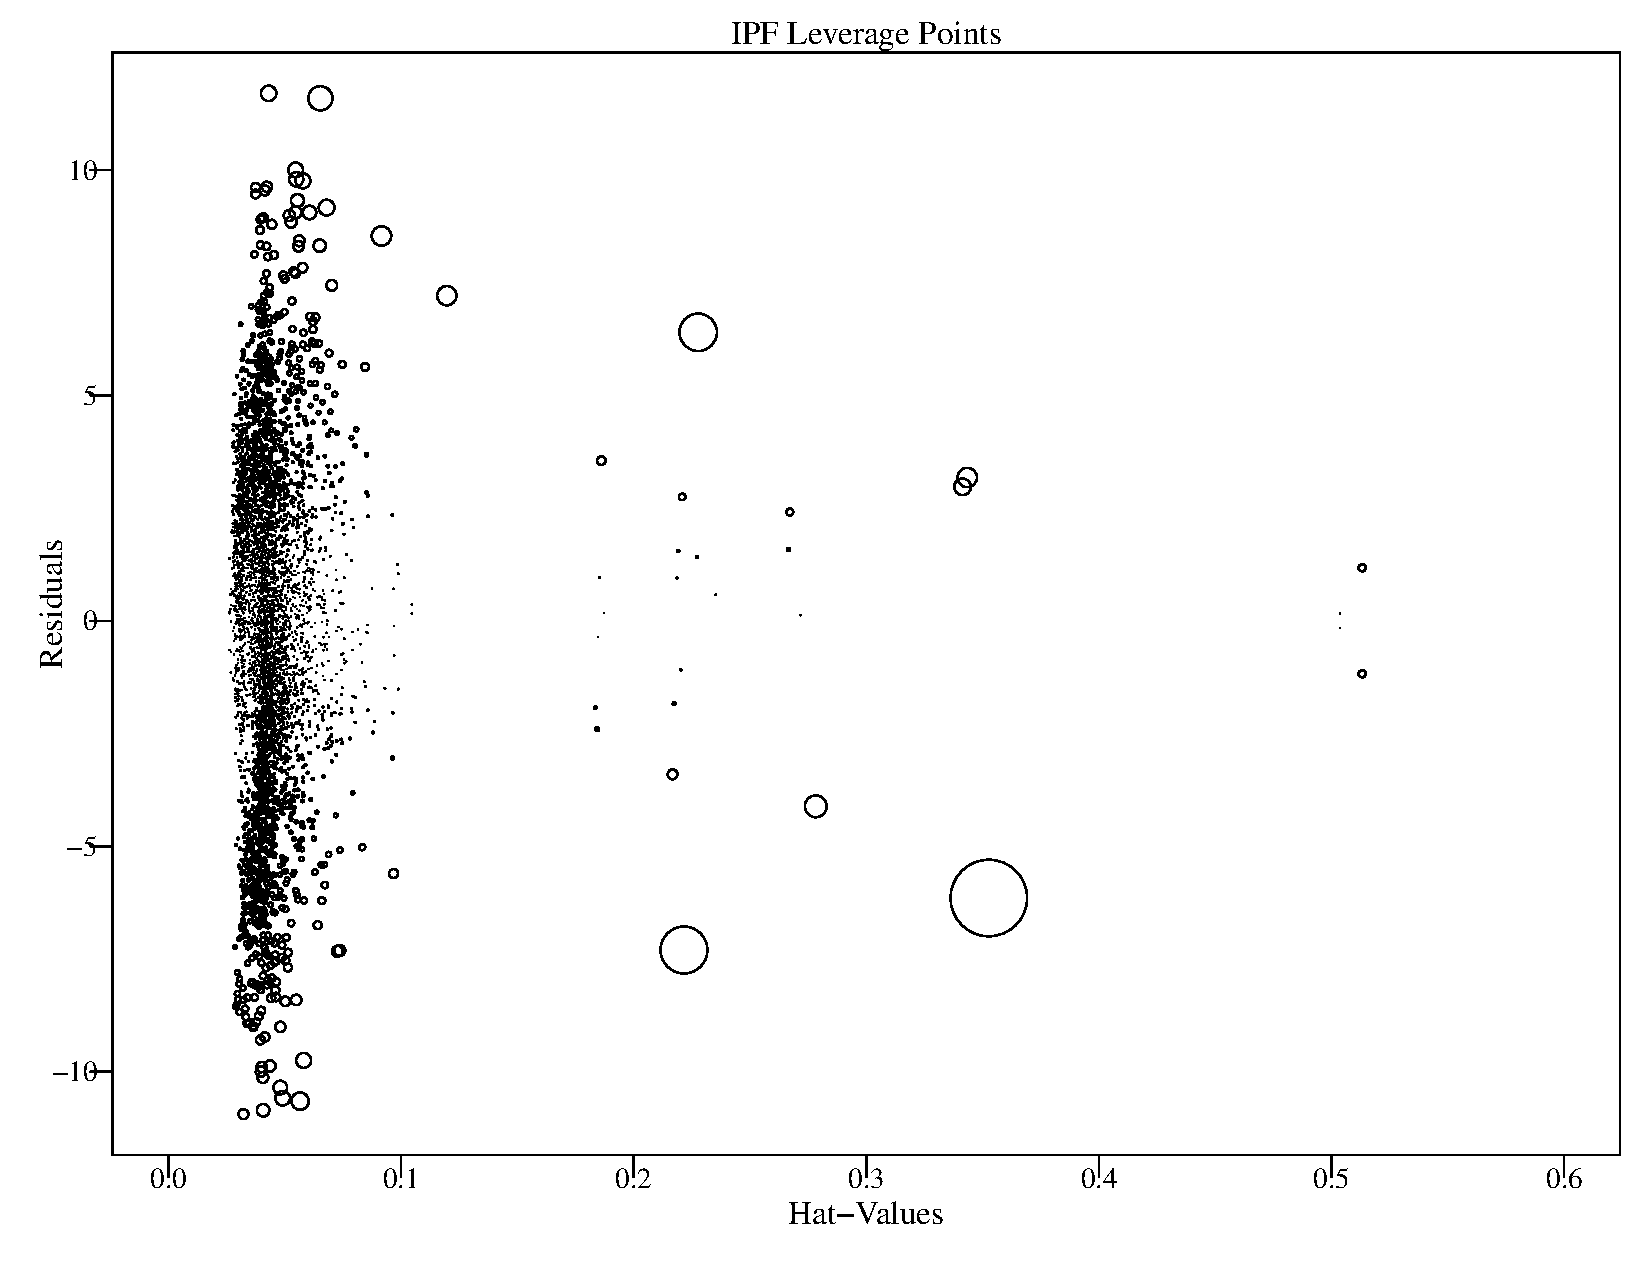
\includegraphics[width = \textwidth]{figs/Rplot_hatvalues_ipf.pdf}
%\caption{Residuals vs. Leverage}\label{fig:hatsipf}
%\end{center}
%\end{figure}

%\newpage
%\begin{figure}[h]
%\begin{center}
%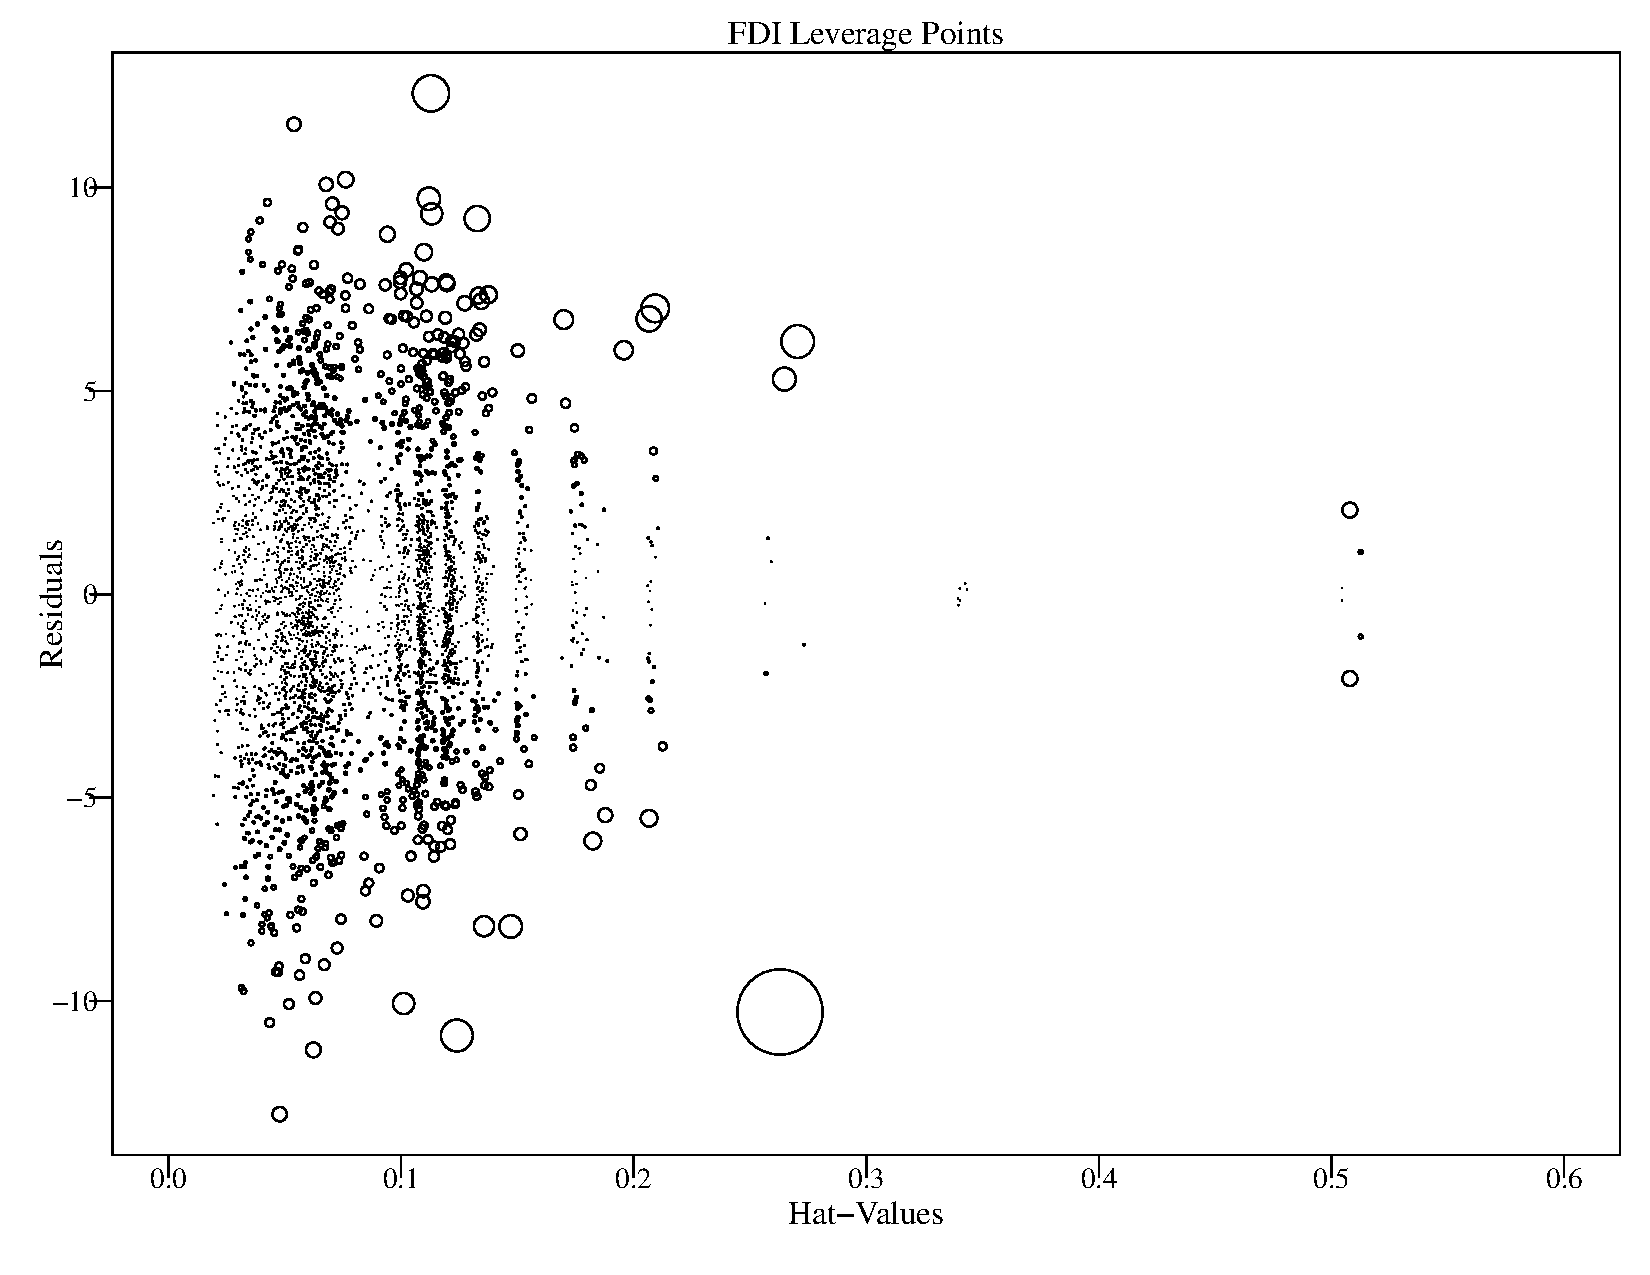
\includegraphics[width = \textwidth]{figs/Rplot_hatvalues_fdi.pdf}
%\caption{Residuals vs. Leverage}\label{fig:hatsfdi}
%\end{center}
%\end{figure}

%\newpage
%\begin{figure}[h]
%\begin{center}
%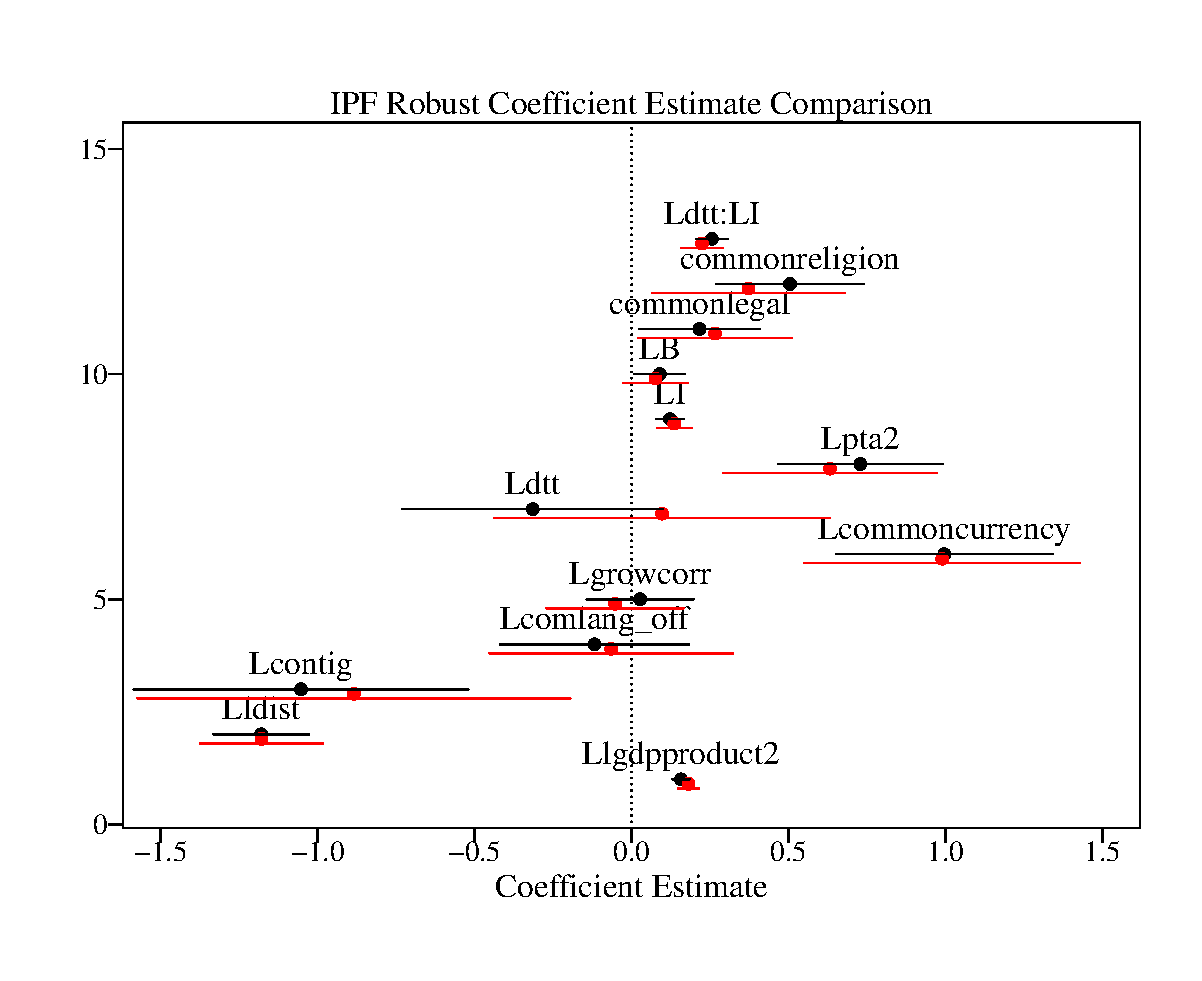
\includegraphics[width = \textwidth]{figs/Rplot_coefficient_estimate_comparison_ipf.pdf}
%\caption{IPF Coefficient Estimate}\label{fig:coefipf}
%\end{center}
%\end{figure} 

%\newpage
%\begin{figure}[h]
%\begin{center}
%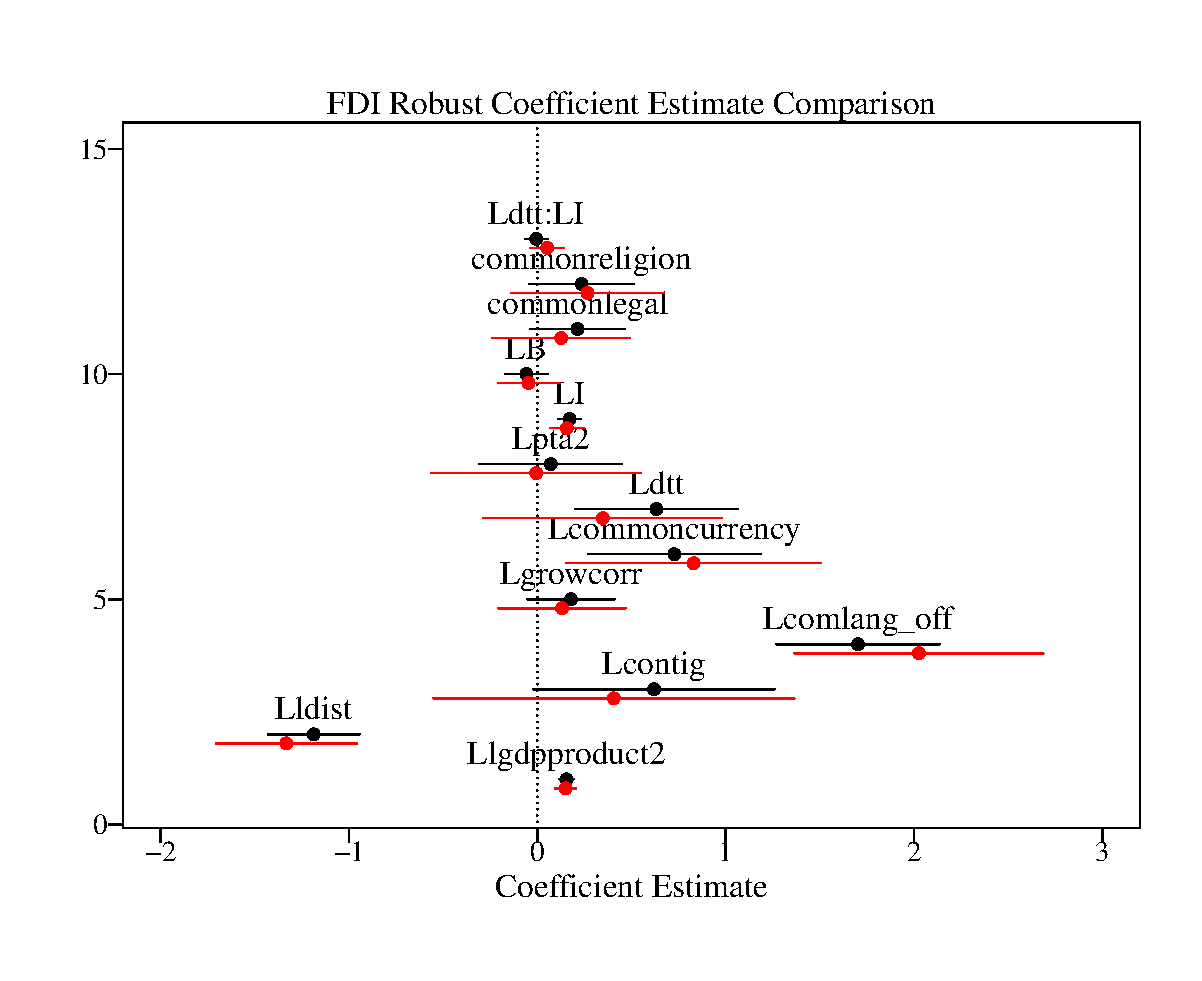
\includegraphics[width = \textwidth]{figs/Rplot_coefficient_estimate_comparison_fdi.pdf}
%\caption{FDI Coefficient Estimate}\label{fig:coeffdi}
%\end{center}
%\end{figure} 

\end{document}